\section{Data Selection and Meson Reconstruction}
\label{sec:dataselection}
This section is about how to reconstruct neutral mesons and the criteria applied in data selection to increase measurement accuracy and is structured in the following way. Section~\ref{sec:eventselection} lists some general restrictions that are also used in Belle note $\#805$, $\#878$, $\#902$ and $\#1347$. Section~\ref{sec:fiducialcut} discusses the selection of fiducial criteria. The assignment of kinematic bins are discussed in section~\ref{sec:kinematicbins}. In the end, $\pi^0$ and $\eta$ reconstruction details are shown. The Monte Carlo used in this note was generated by EvtGen or QQ98 generators and the simulation of Belle detector is based on GEANT3 package \cite{DetectorSimulation}. 

\subsection{Belle Detector Introduction}
Belle detector mainly contains the following parts: Beam pipe, Extreme Forward Calorimeter~(EFC), Silicon Vertex Detector~(SVD), Central Drift Chamber~(CDC), Aerogel Cherenkov Counter~(ACC), Time of Flight Counter (TOF), Electromagnetic Calorimeter (EMCAL), $K_L$ and muon detection system~(KLM).
 
Here focus on the CDC, ACC, TOF and EMCAL. The CDC is used to reconstruct the track of charged particles and precisely measure the momentum of charged particles. It can also be used to measure the energy loss of charged particles $dE/dx$, hence distinguish particles. The TOF measures the flight time of particles and separates particles with different masses. The ACC separates kaons and pions with momentum from $1.2$~GeV$/c$ to $3.5$~GeV$/c$. The purpose of EMCAL is to efficiently detect photons and provide good resolution of energy and position. 

\subsection{Event Selection}
\label{sec:eventselection}
The constraints used for event selection are:
\begin{itemize}
\item To reduce the contribution of neutrino, minimum visible energy is $7$~GeV.  
\item Vertex position is restricted to the range:
\begin{center}
$d_{vertex}<2$~cm   \\
$\lvert z_{vertex}\rvert < 4$~cm
\end{center}
\item Thrust $t>0.8$.
\item PID used in this note:
\begin{itemize}
  \item electron: $\mathcal{L}(e)>0.85$
  \item muon: $\mathcal{L}(\mu)>0.85$
 % \item Kaon: $\nicefrac{\mathcal{L}(p)}{\mathcal{L}(\mathcal{K})}>0.8$
  \item kaon: $\nicefrac{\mathcal{L}(\mathcal{K})}{\mathcal{L}(\pi)}>0.8$
  \item Pion: $\nicefrac{\mathcal{L}(\mathcal{K})}{\mathcal{L}(\pi)}<0.3$
\end{itemize}
\end{itemize}
After applying the PID selection, the efficiency of identified charged pions is around $96.9\%$.

\subsection{Kinematic Bins}
\label{sec:kinematicbins}
As shown in Eq.~\eqref{eqn:FF1}, Collins FF is dependent on $z$ and the transverse momentum $P_t$\footnote{In this analysis, we use $\perp$ to represent the transverse momentum to the real $q\bar{q}$ axis. And the subscript $t$ denotes the transverse momentum to thrust axis.}. Fig.~\ref{fig:zptdistri} shows the distribution of $z$ and $P_t$ with fiducial constraint.
\begin{figure}[H]
  \centering     
  \subfigure[$z$ distribution of mesons]{\label{fig:pi0z}\includegraphics[width=.48\textwidth,natwidth=600,natheight=400]{figure_dataselection/Z_distri.pdf}}
  \subfigure[$P_t$ distribution of mesons]{\label{fig:pi0pt}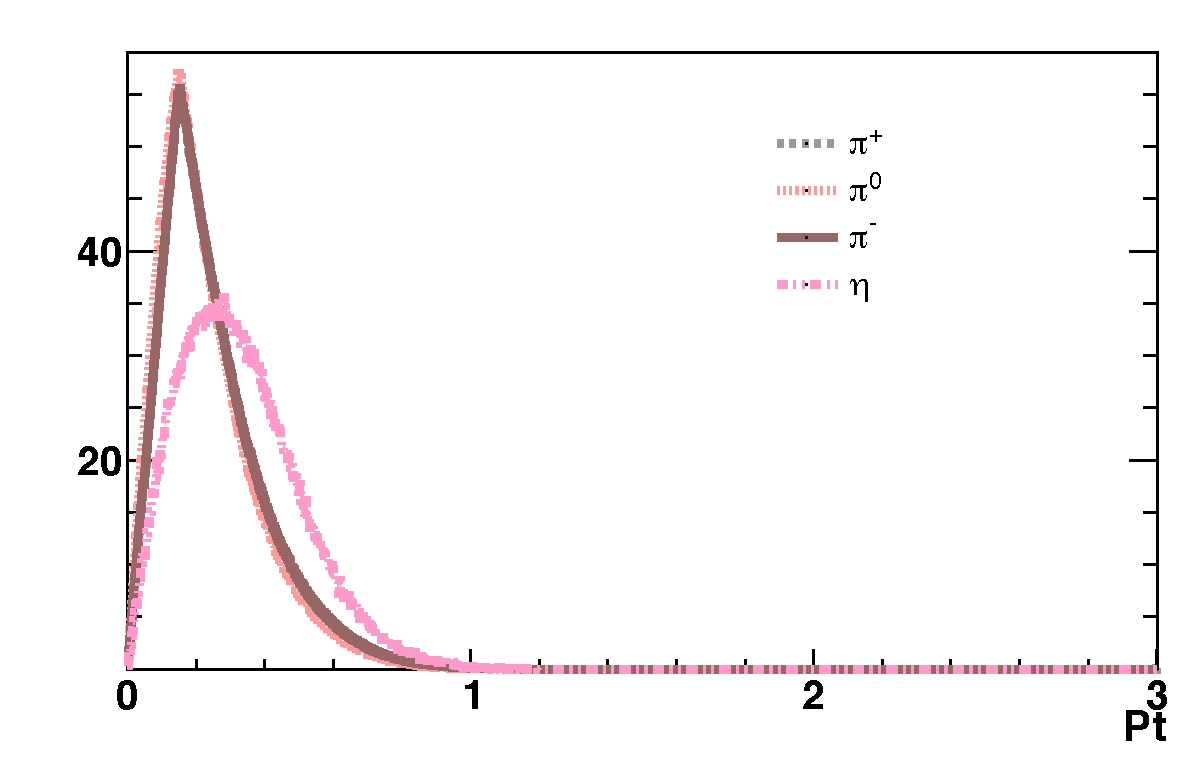
\includegraphics[width=.48\textwidth,natwidth=600,natheight=400]{figure_dataselection/Pt_distri.pdf}}
  \caption{Normalized distribution with kinametic distribution with all event selection, fiducial requirements and the neutral meson reconstruction criteria (see section~\ref{sec:neutralmesonreconstruction}) applied. Left plot is the $z$ distribution of experimental data. The right plot is $P_t$ distribution.}
  \label{fig:zptdistri}
\end{figure}

Hence two kinds of kinematic bins have been studied. In order to study both kinematic dependences the first hadron of the hadron pair is either binned in $z$ or $P_t$ according to the bin boundaries given in Tables~\ref{tab:whatissinglez}~\ref{tab:whatissinglept}. For the neutral/charged mixed hadron pairs, we take the neutral hadron as the first hadron in a hadron pair and the kinematics of first hadron will be labeled with index $1$. While for charged hadron pairs we randomly pick one hadron as the first one. In single kinematic bins the bin number is obtained by $z$ and $P_{t}$ of the first hadron and the dependence on $z_2$ and $P_{t2}$ is integrated out. 
\begin{table}[H]\small
\centering
\begin{tabular}{|l|l|l|l|l|l|l|l|l|}
\hline
$z_1$ bins & 0 &  1 & 2 & 3 & 4 & 5 & 6  \\ \hline
 $z_1$  & {\color{red}0.1$\textup{--}$0.2} & 0.2$\textup{--}$0.3 & 0.3$\textup{--}$0.4 & 0.4$\textup{--}$0.5 & 0.5$\textup{--}$0.6 & 0.6$\textup{--}$0.7 & 0.7$\textup{--}$1  \\ \hline
\end{tabular}
\caption{Bin boundaries for the first-hadron's fractional energy $z_1$ used in the analysis of one-dimensional dependences of the Collins effect.}
\label{tab:whatissinglez}
\end{table}
In the measurement the Collins effect of the lowest $z$ bin is small, and adding this high-statistics bin will dilute the Collins asymmetry. Moreover, in the discussion of kinematics distribution (section~\ref{sec:fiducialcut}) the first $z$ bin has the most detector acceptance effect left. Hence in further study, we only keep events with $0.1<z<0.2$ in $(z_1,z_2)$ bins. For the bins that we integrating over $z$, the threshold will be increased to $0.2$.

\begin{table}[H]\small
\centering
\begin{tabular}{|l|l|l|l|l|l|l|l|l|l|l|l|l|l|l|l|l|l|}
\hline
 $P_{t1}$ bins & 0 &  1 & 2 & 3   \\ \hline
 $P_{t1}$ (GeV)  & 0$\textup{--}$0.15& 0.15$\textup{--}$0.3 & 0.3$\textup{--}$0.5 & 0.5$\textup{--}$3  \\ \hline
\end{tabular}
\caption{Bin boundaries for the first-hadron's transverse momentum $P_{t1}$ used in the analysis of one-dimensional dependences of the Collins effect}
\label{tab:whatissinglept}
\end{table}

Besides integering out the kinematic dependence of the second hadron, we also study the dependence of the asymmetry on both hadrons. In previous charged pion analysis, binning method as shown in Fig.~\ref{fig:comz_mark},\ref{fig:compt_mark} is used because the symmetrical feature of charged pions. 
\begin{figure}[H]
\centering
\begin{minipage}{.5\textwidth}
  \centering
  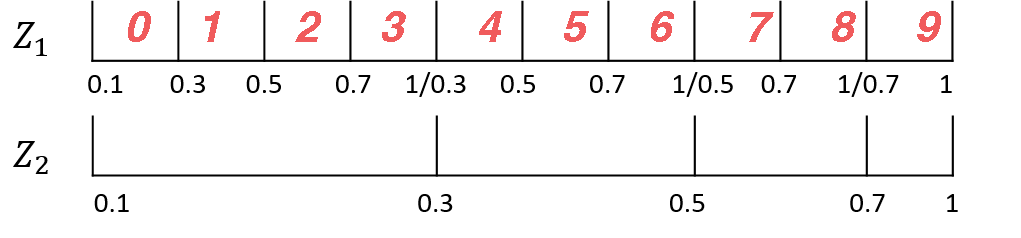
\includegraphics[width=0.95\textwidth,natwidth=610,natheight=642]{figure_dataselection/zbin.pdf}
  \captionof{figure}{$(z_1,z_2)$ bins used in pervious charged pion analysis.}
  \label{fig:comz_mark}
\end{minipage}%
\begin{minipage}{.5\textwidth}
  \centering
  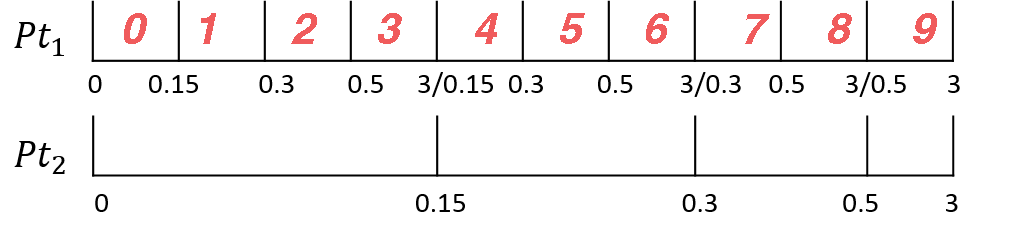
\includegraphics[width=0.95\textwidth,natwidth=610,natheight=642]{figure_dataselection/ptbin.pdf}
  \captionof{figure}{$(P_{t1},P_{t2})$ bins }
  \label{fig:compt_mark}
\end{minipage}
\end{figure}

However, the behavior of $\pi^0$ is different with charged pions and the two hadrons in one hadron pair is not symmetrical. Thus we adopt a more complete binning method as shown in Fig.~\ref{fig:binnings}. To further investigate the dependence of the asymmetry on $z$ and $P_t$ simultaneously, we also used a binning differential in $z$ or $P_t$ as indicated in~\ref{fig:zptbin}.   
\begin{figure}[H]
\captionsetup[subfloat]{farskip=2pt,captionskip=1pt}
\centering
\subfigure[$(z_1,z_2)$ bins]{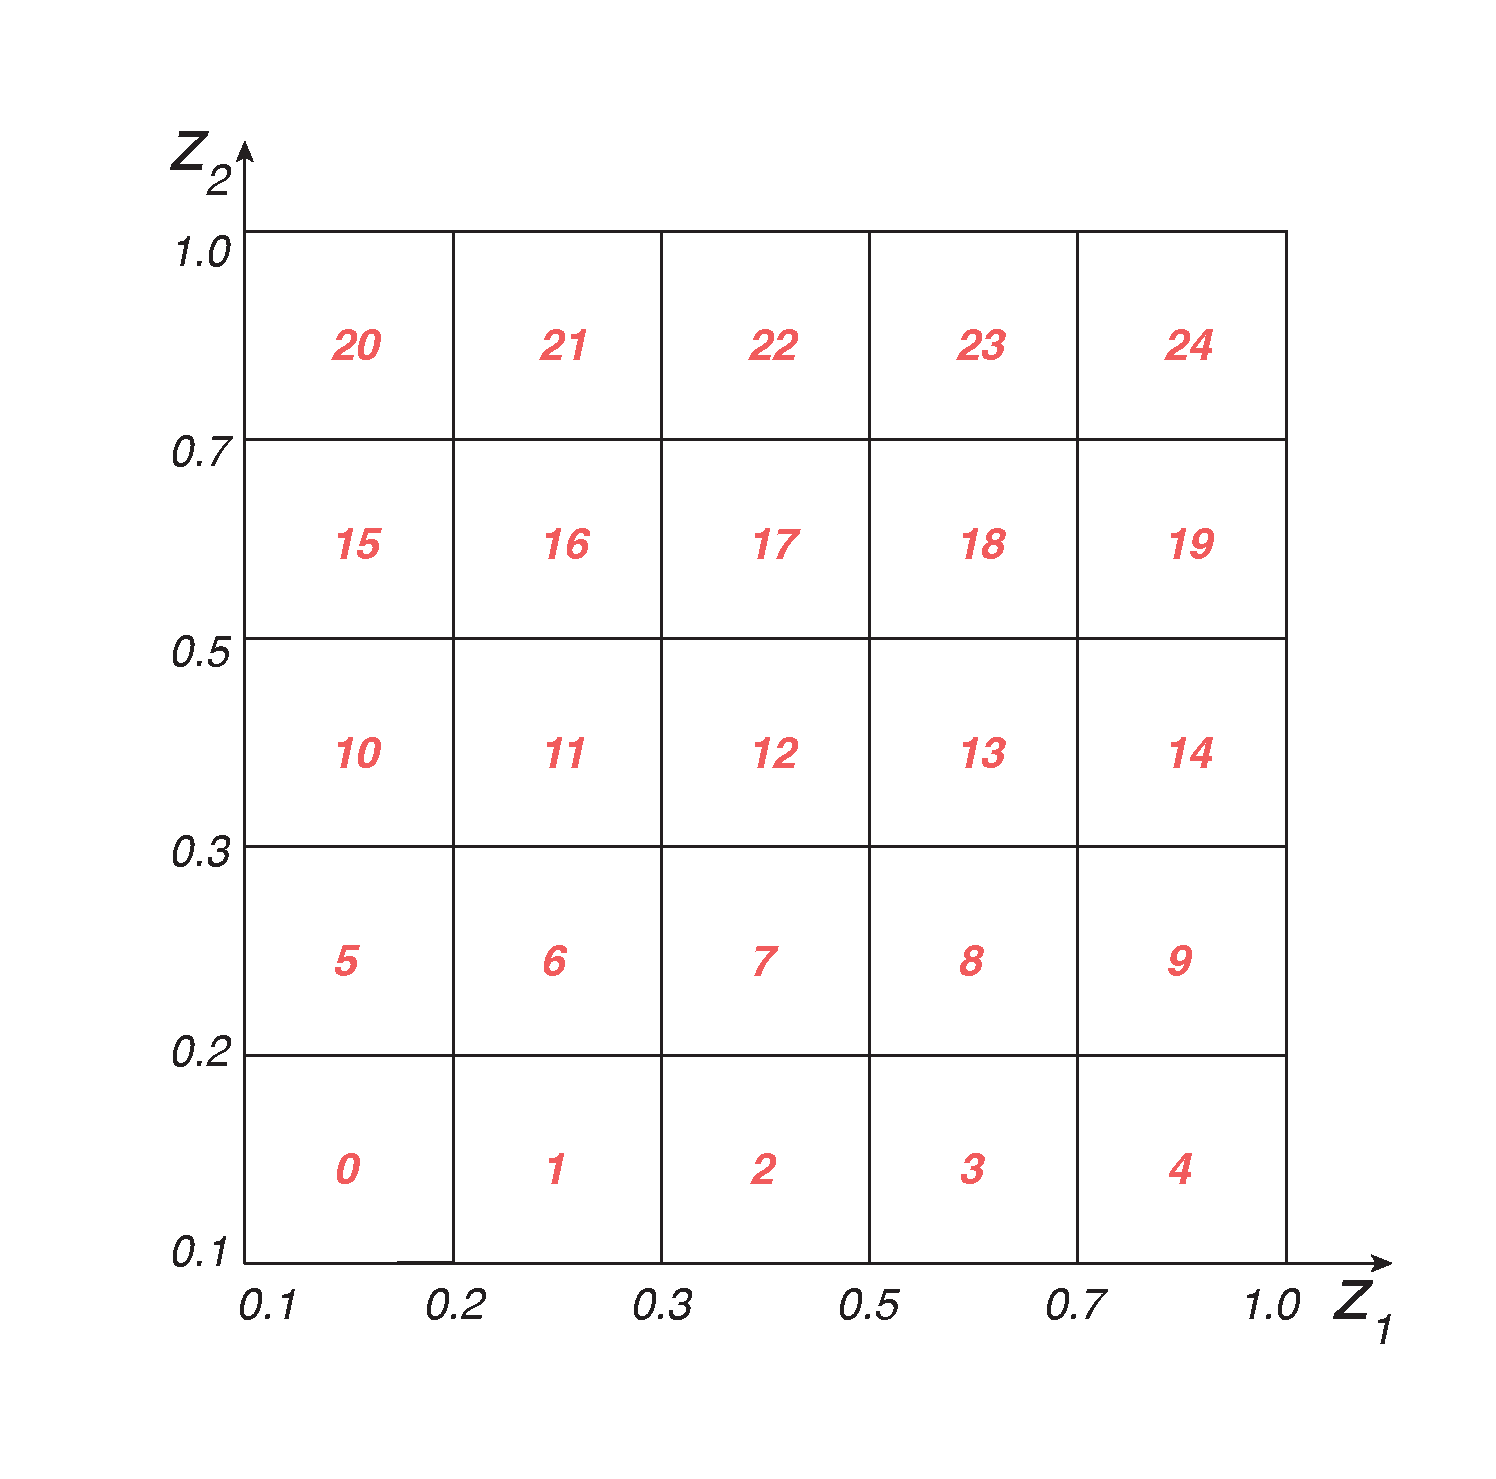
\includegraphics[width=.48\textwidth,natwidth=250,natheight=100]{figure_dataselection/comzbin.pdf}\label{fig:z1z2binning}}
\subfigure[$(P_{t1},P_{t2})$ bins]{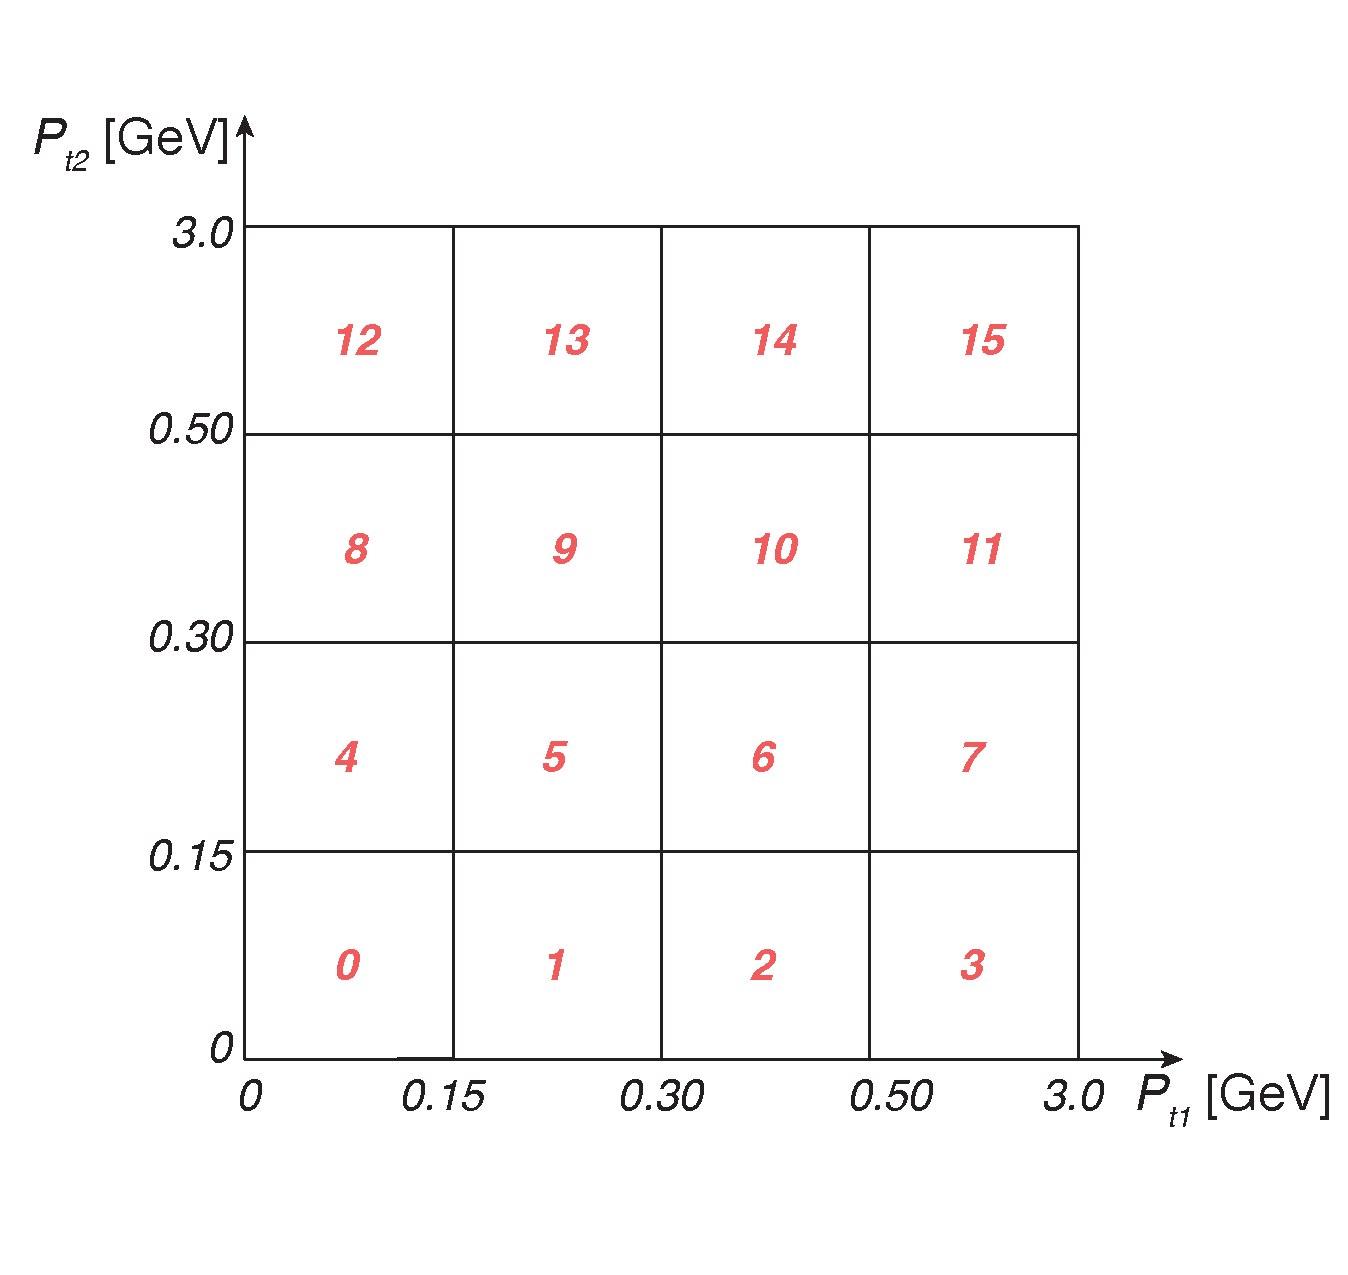
\includegraphics[width=.48\textwidth,natwidth=250,natheight=100]{figure_dataselection/comptbin.pdf}\label{fig:pt1pt2binning}}
\caption{Bin boundaries and numbering for the (hadron1, hadron2) bins. Red numbers are the rank of bins.}
\label{fig:binnings}
\end{figure}

\begin{figure}[H]
    \centering
    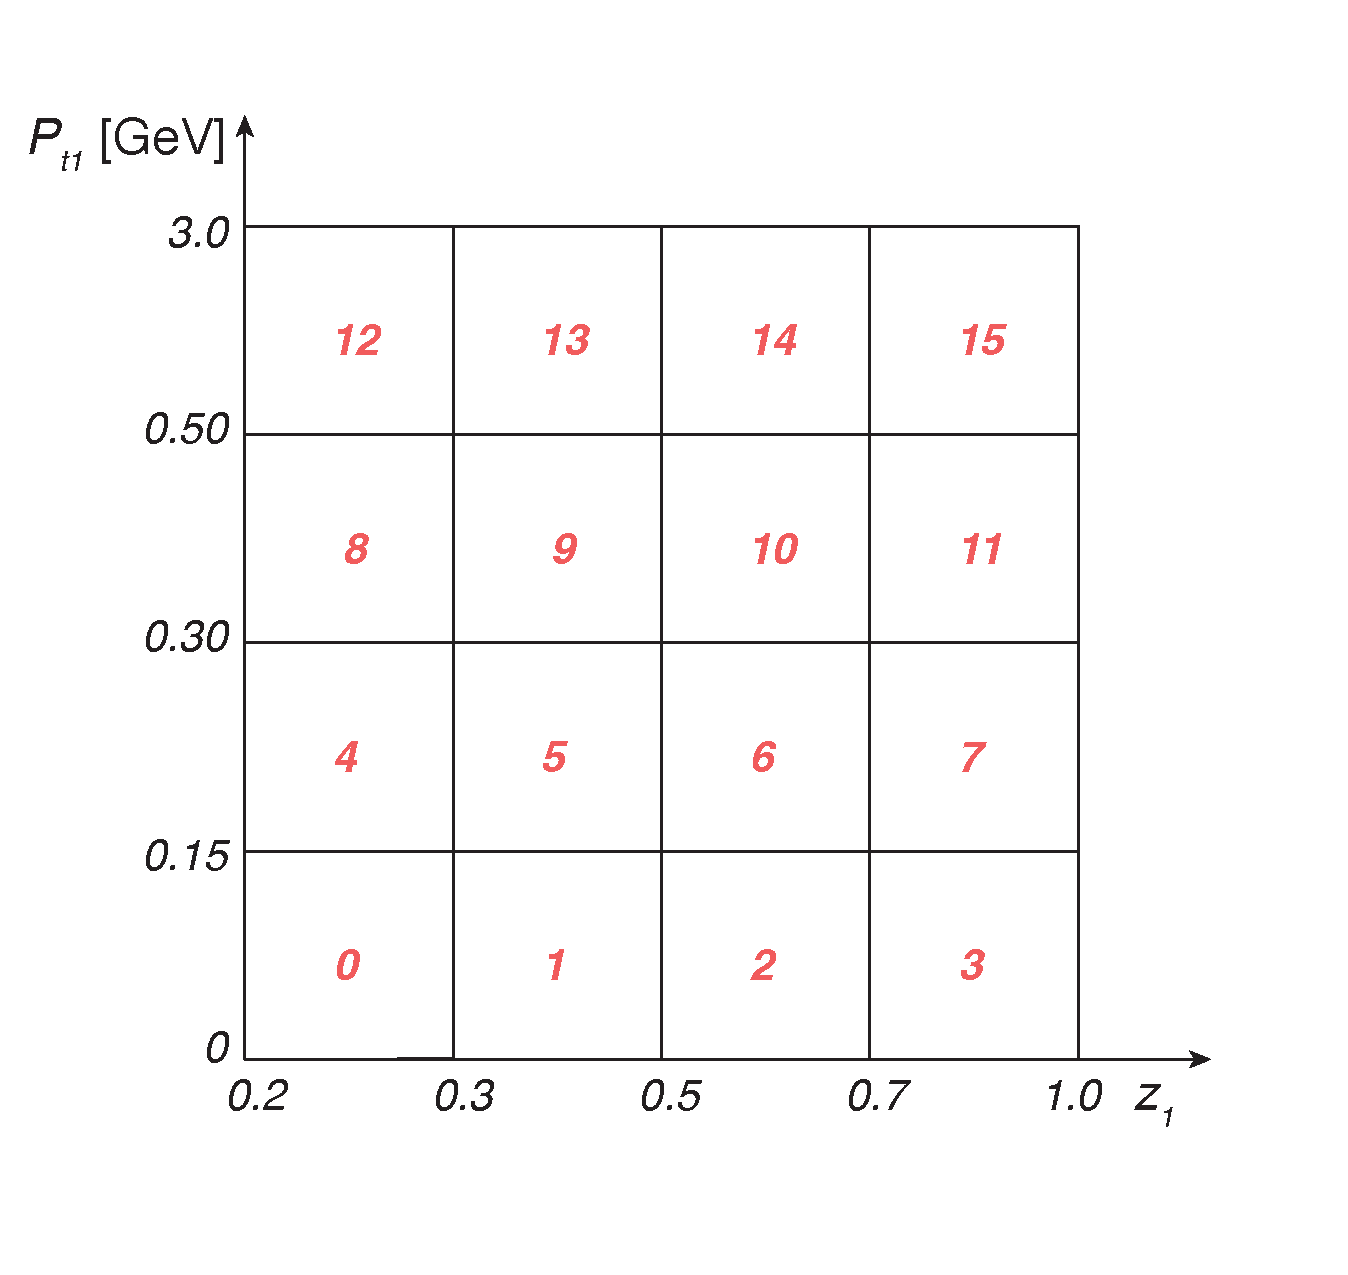
\includegraphics[width=0.6\textwidth,natwidth=250,natheight=100]{figure_dataselection/zptbin.pdf}
    \caption{Bin boundaries and numbering for the 2d binning of the neutral-meson kinematics $z$ and $P_t$.}
    \label{fig:zptbin}
\end{figure}

\subsection{Fiducial and Energy Constraints for Hadron Selection}
\subsubsection{Fiducial Constraints}
\label{sec:fiducialcut}
Certain fiducial constraints are applied to guarantee that all particles used in the analysis are captured in the barrel electromagnetic calorimeter~(EMCAL) as in Fig.~\ref{fig:2} and all particles must be symmetrically distributed around the thrust axis to avoid false Collins asymmetry. In CMS, hadrons and gammas should be limited within $0.84<\theta^{CMS}<2.53$~rad which corresponds to the barrel EMCAL, where $\theta^{CMS}$ is the angle between momentum direction and the $e^+e^-$ axis, to minimize detector edge effects. All angles related to fiducial constraints are measured in the CMS.
\begin{figure}[H]
  \centering
  \includegraphics[width=0.8\textwidth,natwidth=610,natheight=642]{figure_dataselection/EMCAL.pdf}
  %\includegraphics[scale=.3,keepaspectratio]{EMCAL.pdf}
  \caption{Configuration of Belle electromagnetic calorimeter~\cite{BelleDetector}}
  \label{fig:2}
\end{figure}
The fiducial constraints, together with energy constraints of neutral meson reconstruction, are used to retrieve the optimized set of constraints based on the FOM, $\nicefrac{S}{\sqrt{N}}$, of Monte Carlo data. The following cuts are considered:
\begin{itemize}
  \item Opening angle (OA): $<0.4$~rad, $<0.5$~rad, $<0.6$~rad.
  \item Photon Energy:
    \begin{itemize}
      \item $\pi^{0}$: $50$~MeV, $100$~MeV, $150$~MeV. 
      \item $\eta$: $150$~MeV, $200$~MeV, $250$~MeV, $300$~MeV, $400$~MeV. 
    \end{itemize}
  \item Photon Energy asymmetry $A_{\gamma\gamma}=\frac{|\gamma_1-\gamma_2|}{\gamma_1+\gamma_2}$ : $<0.8$ ,$<0.9$, $<1$.
\end{itemize}
\begin{figure}[H]
  \centering
  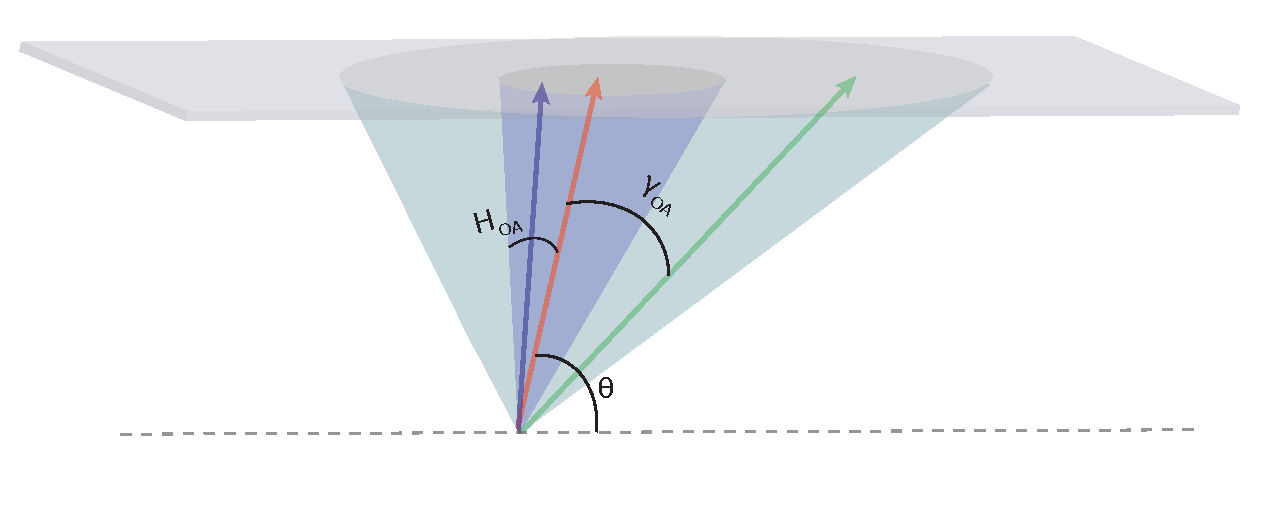
\includegraphics[width=0.95\textwidth,natwidth=610,natheight=642]{figure_dataselection/OA.pdf}
  \captionof{figure}{Fiducial constraint illustration in the CMS system. The red line is thrust axis. The outer cone stand for the boundary of $\gamma$s and inner cone for hadron. To make sure that all $\gamma$s are captured by ECL, the value of $\theta^{CMS}_{thrust}\pm \gamma_{OA}$ should fall in $\theta^{CMS}$ range $0.84~\text{rad}<\theta^{CMS}_{thrust}<2.53~\text{rad}$.}
  \label{fig:FiducialCut}
\end{figure}
Here, OA is the angle between hadrons/photons and the thrust axis. This constraint, the range of the polar angle $\theta_{thrust}^{CMS}$ of the thrust axis to the beam axis in the CMS is adjusted such that even at maximal OA tracks and photons are contained in the allowed polar-angle range given above. For example, if the maximum OA is $0.4$~rad, the thrust direction is limited within $1.24~\text{rad}<\theta^{CMS}_{thrust}<2.13~\text{rad}$.  Tighter boundary of OA leaves more room for thrust range at the expense of the yield of hadrons, and vice versa as shown in Fig.~\ref{fig:OAs}. We apply the same OA in the hadrons and gammas selection as a preliminary criterion and further study of hadron OA will be discussed later.
\begin{figure}[h]
  \centering     %%% not \center
  \subfigure[$\pi^0$ to thrust angle]{\label{fig:a}\includegraphics[width=60mm]{figure_dataselection/pi0_OA.eps}}
  \subfigure[$\eta$ to thrust angle]{\label{fig:b}\includegraphics[width=60mm]{figure_dataselection/eta_OA.eps}}
  \caption{$H_{OA}$ distribution under various $\gamma_{OA}$ constraints, different color lines represent different $\gamma_{OA}$ constraints. For example, the $\gamma_{OA}$ constraint for red solid line is 0.3~rad. It can be seen that with the decrease of $\gamma$ range, the width of hadron distribution becomes thinner.}
  \label{fig:OAs}
\end{figure}

The $\gamma$ energy threshold and energy asymmetry are studied to reduce the background contribution. Higher threshold leads to purer data at the expense of yield loss. Similarly, tighter energy asymmetry requirement also improves the signal purity as shown in Fig~\ref{fig:photon_asymmetry}, but reduces the yield.
\begin{figure}[H]
\centering
  \subfigure[]{\label{fig:photon_asymmetry1}\includegraphics[width=.48\textwidth,natwidth=250,natheight=100]{figure_dataselection/pi0_asy_plot_Z3.pdf}}
  \subfigure[]{\label{fig:photon_asymmetry2}\includegraphics[width=.48\textwidth,natwidth=250,natheight=100]{figure_dataselection/pi0_asy_plot_Z6.pdf}}
  \caption{Two examples of energy asymmetry $A_{\gamma\gamma}$. Left plot is $0.4<z<0.5$ and right plot is $0.7<z<1.0$. In each plot, blue line is the signal energy asymmetry and purple line is the background energy asymmetry. To make the plots, the invariant mass of reconstructed $\pi^0$ are restricted in the range of $0.1$~GeV$\textup{--}0.18$~GeV to avoid contribution of $\eta$ or other irrelevant background. As MC data is used in this plot, the signal and background events are distinguished by the particle ID of the reconstructed particles as well as the ID of their parents.}
\label{fig:photon_asymmetry}
\end{figure}

Table~\ref{tab:FOM} show the optimized constraints for each kinematic bins. Most bins of $\pi^0$ have the same optimized constraints, namely the photon energy threshold $50$~MeV, no photon energy asymmetry cut and OA constraint $0.5$, and these constraints are chosen as our data selection criteria. For other bins, comparisons are made to confirm that the FOMs of selected criteria of that bin approximate the optimized FOM. The same approach is used for $\eta$ and the final selection criteria for $\eta$ can be found at Table~\ref{tab:constrain}.%includes the photon energy threshold $250$~MeV, no photon energy asymmetry cut and OA constraint $0.5$. With $z<0.3$ the purity of $\eta$ is below $30\%$ and thus it is required that $z>0.3$ for $\eta$ mesons. 
\begin{table}[H]
\begin{tabular}{|p{1.3cm}|l|l|l|l|l|l|l|l|l|l|l|l|l|}
\hline
Bin & $E_{\gamma}$~MeV & $A_{\gamma\gamma}$ & OA \\ \hline
$z_0$ & 0.05 & 0.8 & 0.6 \\\hline
$z_1$ & 0.05 & 0.9 & 0.5 \\\hline
$z_2$ & 0.05 & 1 & 0.5 \\\hline
$z_3$ & 0.05 & 1 & 0.5 \\\hline
$z_4$ & 0.10 & 1 & 0.5 \\\hline
$z_5$ & 0.05 & 1 & 0.5 \\\hline
$z_6$ & 0.05 & 1 & 0.5 \\\hline
$P_{t0}$ & 0.05 & 1 & 0.5 \\\hline
$P_{t1}$ & 0.05 & 1 & 0.5 \\\hline
$P_{t2}$ & 0.10 & 1 & 0.5 \\\hline
$P_{t3}$ & 0.05 & 1 & 0.6 \\\hline
\end{tabular}
%\caption{Constraints that generate optimized FOM for $\pi^{0}$.}
%\label{tab:pi0FOM}
\quad
\begin{tabular}{|p{1.3cm}|l|l|l|l|l|l|l|l|l|l|l|l|l|}
\hline
Bin & $E_{\gamma}$~MeV & $A_{\gamma\gamma}$ & OA \\ \hline
$z_0$ &  &  &  \\\hline
$z_1$ &  &  &  \\\hline
$z_2$ & 0.15 & 1 & 0.5 \\\hline
$z_3$ & 0.25 & 1 & 0.5 \\\hline
$z_4$ & 0.25 & 1 & 0.5 \\\hline
$z_5$ & 0.25 & 1 & 0.5 \\\hline
$z_6$ & 0.25 & 1 & 0.5 \\\hline
$P_{t0}$ & 0.20 & 1 & 0.5 \\\hline
$P_{t1}$ & 0.20 & 1 & 0.5 \\\hline
$P_{t2}$ & 0.15 & 1 & 0.5 \\\hline
$P_{t3}$ & 0.25 & 1 & 0.5 \\\hline
\end{tabular}
\caption{Constraints that generate optimized FOM for $\pi^0$~(left) and $\eta$~(right).}
\label{tab:FOM}
\end{table}

Fig.~\ref{fig:FiducialCut} shows the hadron/photon to thrust opening angles that will be used to do fiducial constraint. Our previous study shows that the optimized criteria for OA is $0.5$ for hadrons/photons. However, as in the double ratio method the cancellation of detector effect implies the requirement of identical kinematic distribution for all hadrons to somewhat make up for that loss of acceptance for neutral mesons. The choice made here is to equalize kinematic distributions between neutral and charged mesons. In \cref{fig:kine_distri1,fig:kine_distri2,fig:kine_distri3,fig:kine_distri4} we can see better agreement of the kinematic distribution of pions under tighter $H_{OA}$ constraints. More plots could be found in section~\ref{sec:kinedistri_pi0}~\ref{sec:kinedistri_eta}.
\begin{figure}[H]
\captionsetup[subfloat]{farskip=2pt,captionskip=1pt}
\centering
\subfigure[$H_{OA}<0.3$]{\includegraphics[width=.31\textwidth,natwidth=250,natheight=100]{figure_fiducial/had0.3/Pt_distri_for_zbin_1_norm_had03.pdf}\label{fig:kine_distri11}}
\subfigure[$H_{OA}<0.4$]{\includegraphics[width=.31\textwidth,natwidth=250,natheight=100]{figure_fiducial/had0.4/Pt_distri_for_zbin_1_norm_had04.pdf}\label{fig:kine_distri12}}
\subfigure[$H_{OA}<0.5$]{\includegraphics[width=.31\textwidth,natwidth=250,natheight=100]{figure_fiducial/had0.5/Pt_distri_for_zbin_1_norm_had05.pdf}\label{fig:kine_distri13}}
\caption{Normalized $P_t$ distribution of pions for $0.2<z<0.3$}
\label{fig:kine_distri1}
\end{figure}

\begin{figure}[H]
\captionsetup[subfloat]{farskip=2pt,captionskip=1pt}
\centering
\subfigure[$H_{OA}<0.3$]{\includegraphics[width=.31\textwidth,natwidth=250,natheight=100]{figure_fiducial/had0.3/Pt_distri_for_ptbin_1_norm_had03.pdf}\label{fig:kine_distri21}}
\subfigure[$H_{OA}<0.4$]{\includegraphics[width=.31\textwidth,natwidth=250,natheight=100]{figure_fiducial/had0.4/Pt_distri_for_ptbin_1_norm_had04.pdf}\label{fig:kine_distri22}}
\subfigure[$H_{OA}<0.5$]{\includegraphics[width=.31\textwidth,natwidth=250,natheight=100]{figure_fiducial/had0.5/Pt_distri_for_ptbin_1_norm_had05.pdf}\label{fig:kine_distri23}}
\caption{Normalized $P_t$ distribution of pions for $0<P_{t}<0.15$}
\label{fig:kine_distri2}
\end{figure}

\begin{figure}[H]
\captionsetup[subfloat]{farskip=2pt,captionskip=1pt}
\centering
\subfigure[$H_{OA}<0.3$]{\includegraphics[width=.31\textwidth,natwidth=250,natheight=100]{figure_fiducial/had0.3/Z_distri_for_zbin_0_norm_had03.pdf}\label{fig:kine_distri31}}
\subfigure[$H_{OA}<0.4$]{\includegraphics[width=.31\textwidth,natwidth=250,natheight=100]{figure_fiducial/had0.4/Z_distri_for_zbin_0_norm_had04.pdf}\label{fig:kine_distri32}}
\subfigure[$H_{OA}<0.5$]{\includegraphics[width=.31\textwidth,natwidth=250,natheight=100]{figure_fiducial/had0.5/Z_distri_for_zbin_0_norm_had05.pdf}\label{fig:kine_distri33}}
\caption{Normalized $z$ distribution of pions for $0.1<z<0.2$}
\label{fig:kine_distri3}
\end{figure}

\begin{figure}[H]
\captionsetup[subfloat]{farskip=2pt,captionskip=1pt}
\centering
\subfigure[$H_{OA}<0.3$]{\includegraphics[width=.31\textwidth,natwidth=250,natheight=100]{figure_fiducial/had0.3/Z_distri_for_ptbin_1_norm_had03.pdf}\label{fig:kine_distri41}}
\subfigure[$H_{OA}<0.4$]{\includegraphics[width=.31\textwidth,natwidth=250,natheight=100]{figure_fiducial/had0.4/Z_distri_for_ptbin_1_norm_had04.pdf}\label{fig:kine_distri42}}
\subfigure[$H_{OA}<0.5$]{\includegraphics[width=.31\textwidth,natwidth=250,natheight=100]{figure_fiducial/had0.5/Z_distri_for_ptbin_1_norm_had05.pdf}\label{fig:kine_distri43}}
\caption{Normalized $z$ distribution of pions for $0.15<P_t<0.3$}
\label{fig:kine_distri4}
\end{figure}

\begin{figure}[H]
\captionsetup[subfloat]{farskip=2pt,captionskip=1pt}
\centering
\subfigure[$H_{OA}<0.3$]{\includegraphics[width=.31\textwidth,natwidth=250,natheight=100]{figure_fiducial/had0.3_z0.3/Pt_distri_for_zbin_2_norm_had03z03.pdf}\label{fig:kine_distri51}}
\subfigure[$H_{OA}<0.4$]{\includegraphics[width=.31\textwidth,natwidth=250,natheight=100]{figure_fiducial/had0.4_z0.3/Pt_distri_for_zbin_2_norm_had04z03.pdf}\label{fig:kine_distri52}}
\caption{Normalized $P_t$ distribution of eta and pions for $0.3<z<0.4$}
\label{fig:kine_distri5}
\end{figure}

\begin{figure}[H]
\captionsetup[subfloat]{farskip=2pt,captionskip=1pt}
\centering
\subfigure[$H_{OA}<0.3$]{\includegraphics[width=.31\textwidth,natwidth=250,natheight=100]{figure_fiducial/had0.3_z0.3/Pt_distri_for_ptbin_1_norm_had03z03.pdf}\label{fig:kine_distri61}}
\subfigure[$H_{OA}<0.4$]{\includegraphics[width=.31\textwidth,natwidth=250,natheight=100]{figure_fiducial/had0.4_z0.3/Pt_distri_for_ptbin_1_norm_had04z03.pdf}\label{fig:kine_distri62}}
\caption{Normalized $P_t$ distribution of eta and pions for $0.15<P_t<0.3$}
\label{fig:kine_distri6}
\end{figure}

\begin{figure}[H]
\captionsetup[subfloat]{farskip=2pt,captionskip=1pt}
\centering
\subfigure[$H_{OA}<0.3$]{\includegraphics[width=.31\textwidth,natwidth=250,natheight=100]{figure_fiducial/had0.3_z0.3/Z_distri_for_zbin_3_norm_had03z03.pdf}\label{fig:kine_distri71}}
\subfigure[$H_{OA}<0.4$]{\includegraphics[width=.31\textwidth,natwidth=250,natheight=100]{figure_fiducial/had0.4_z0.3/Z_distri_for_zbin_3_norm_had04z03.pdf}\label{fig:kine_distri72}}
\caption{Normalized $z$ distribution of eta and pions for $0.4<z<0.5$}
\label{fig:kine_distri7}
\end{figure}

\begin{figure}[H]
\captionsetup[subfloat]{farskip=2pt,captionskip=1pt}
\centering
\subfigure[$H_{OA}<0.3$]{\includegraphics[width=.31\textwidth,natwidth=250,natheight=100]{figure_fiducial/had0.3_z0.3/Z_distri_for_ptbin_3_norm_had03z03.pdf}\label{fig:kine_distri81}}
\subfigure[$H_{OA}<0.4$]{\includegraphics[width=.31\textwidth,natwidth=250,natheight=100]{figure_fiducial/had0.4_z0.3/Z_distri_for_ptbin_3_norm_had04z03.pdf}\label{fig:kine_distri82}}
\caption{Normalized $z$ distribution of eta and pions for $0.5<P_t<3$}
\label{fig:kine_distri8}
\end{figure}

From the above graphs, we choose the maximum value of hadron to thrust opening angle as $0.3$ to get the equalized hadron kinematics distributions. 

\subsubsection{\texorpdfstring{Energy Constraint for $\gamma$ and mesons}{Energy Constraint for gamma and mesons}}
\label{sec:energyconstraint}
The following energy constraints are adopted to reconstruct neutral mesons:
\begin{itemize}
\item $\gamma$ energy constraint $50$~MeV for $\pi^0$, $150$~MeV for $\eta$.
\item $z>0.1$ for hadrons forming double ratios that contain $\pi^0$.\footnote{For the kinematic bins that $z$ would be integrated, the threshold is increased to $z>0.2$. More details can be found in section~\ref{sec:kinematicbins}.}
\item $z>0.3$ for hadrons forming double ratios that contain $\eta$. 
\end{itemize}

In summary, the principle behind the fiducial constraints summarized in Table~\ref{tab:constrain} is that all particles are captured by the barrel EMCAL and the hadrons are accepted symmetrically around thrust axis indicated by similar kinematic distributions. With $\gamma_{OA}<0.5$ we obtained highest FOM, and $H_{OA}$ is set to satisfy the requirement of similar geometric acceptance. Fig.~\ref{fig:differentthetarange} compares the $\phi_1+\phi_2$ distribution for $\pi^0\pi^++\pi^0\pi^-$ paris with and without applying the set of fiducial constraints. It can be seen that after applying fiducial constraint, the amplitude of $R_{12}$ reduces significantly. This result also illustrates that  most of the false asymmetry comes from the detector effect. Last but not least it should be noted that all these studies were performed on the Belle MC sample using the PYTHIA $6.1$. In MC simulation the Collins effect was not installed thus the $cos$ shape distribution, the so-called false asymmetry, mainly arises from detector acceptance effect. Thus MC simulation provides good examination in particular for the false asymmetries dominated by acceptance effect.

\begin{figure}[h]
    \centering
    \includegraphics[width=0.8\textwidth,natwidth=610,natheight=642]{figure_dataselection/DetectorEffect.pdf}
    \caption{The normalized ratio $R_{12}$ for $\pi^0\pi^++\pi^0\pi^-$ with $0.3<z<0.4$ using MC data. The red histogram stands for the situation that no thrust or hadron direction cuts are applied. The blue histogram uses the criterion $\gamma_{OA} <0.3~\text{rad}$, $H_{OA}<0.5~\text{rad}$ and $1.34~\text{rad}<\theta^{CMS}_{thrust}<2.03~\text{rad}$.}
    \label{fig:differentthetarange}
\end{figure}

\begin{table}[H]\small
\centering
\begin{tabular}{|l|l|l|l|l|l|l|l|l|}
\hline
constrants &   \\ \hline
$E_\gamma$~($\pi^0$) & $E_\gamma >50$~MeV \\ \hline
$E_\gamma$~($\eta$) & $E_\gamma >250$~MeV \\ \hline
$z$~($\pi^0$) & $z>0.1$ \\ \hline
$z$~($\eta$) & $z>0.3$ \\ \hline
$\gamma_{OA}$ & 0.5 \\ \hline
$H_{OA}$ & 0.3 \\ \hline
$\theta$ &  $1.34~\text{rad}$\textup{--}$ 2.03~\text{rad}$ \\ \hline
\end{tabular}
\caption{Fiducial and energy constraints.}
\label{tab:constrain}
\end{table}

\subsection{Neutral Meson Reconstruction}
\label{sec:neutralmesonreconstruction}
In order to reconstruct neutral mesons efficiently, several energy constraints are adopted. Section~\ref{sec:energyconstraint} shows the energy criteria that are used to reduce background and maintain yield in the meanwhile. The fitting process of reconstructed invariant mass is discussed in section~\ref{sec:pi0fitsection}~\ref{sec:etafitsection}. To further improve the signal ratio, mass windows are studies in~\ref{sec:masswindow}.

\subsubsection{\texorpdfstring{Invariant Mass fit of $\pi^0$}{pi0 fit}}
\label{sec:pi0fitsection}
The intuitive method to fit $\pi^0$ is using a fitting function consisting of a polynomial and a Gaussian function. Polynomial distribution function is a good estimate of background while Gaussian is normally used to fit signal. However, here we use Crystal Ball function to fit signals because it has asymmetrical tails which can describe the left tail caused by $\gamma$ decay~($gamma\rightarrow ee$).

Moreover, the background of Monte Carlo can be used to simulate and estimate the background of experimental data. We take the discrepancy of those two fitting methods as a source of the systematic uncertainty.
\subsubsection{Fit with Crystal Ball Function}
We use the polynomial function of degree 5 and Crystal Ball function to describe the background and signal. Crystal ball function is defined as~\cite{CrystalBallFunc}
\begin{subequations}
\begin{align}
f(x;\alpha,n,\bar x,\sigma) & = N \cdot \begin{cases} \exp(- \frac{(x - \bar x)^2}{2 \sigma^2}), & \mbox{for }\frac{x - \bar x}{\sigma} > -\alpha \\
 A \cdot (B - \frac{x - \bar x}{\sigma})^{-n}, & \mbox{for }\frac{x - \bar x}{\sigma} \leqslant -\alpha \end{cases}\\
A & = \left(\frac{n}{\left| \alpha \right|}\right)^n \cdot \exp\left(- \frac {\left| \alpha \right|^2}{2}\right), \\
B &= \frac{n}{\left| \alpha \right|}  - \left| \alpha \right|,\\
%N &=\frac{1}{\sigma(C+D)},
%C &=\frac{n}{\left|\alpha \right| \cdot \frac{1}{n-1} \cdot \exp(-\frac{\left| \alpha \right|^2}{2}),\\
%D &=\sqrt{\frac{\pi}{2}}(1+\DeclareMathOperator\erf{erf}(\frac{\left| \alpha \right|}{\sqrt{2}}))
N &= \frac{1}{\sigma (C + D)}</math>\\
C &= \frac{n}{\left| \alpha \right|} \cdot \frac{1}{n-1} \cdot \exp\left(- \frac {\left| \alpha \right|^2}{2}\right) \\
D &= \sqrt{\frac{\pi}{2}} \left(1 + \operatorname{erf}\left(\frac{\left| \alpha \right|}{\sqrt 2}\right)\right) \\
\end{align}
\label{eqn:crystalball}
\end{subequations}
Figure~\ref{fig:pi0_crystalfit} contains some fitting examples. More plots could be found at Appendix~\ref{sec:cryfitpi0}. The vertical black dash line in the plots are boundaries of signal mass window that we will discuss in section~\ref{sec:masswindow}. In those plots the fitting result (blue line) shows good agreement with experimental data except some slight differences in sideband regions. 
\begin{figure}[H]
  \centering     
  \subfigure[$\pi^0$ invariant mass fit, $0<P_t<0.15$]{\label{fig:pi0crystalfit_1}\includegraphics[width=.48\textwidth,natwidth=600,natheight=400]{figure_dataselection/pi0_crystalfit_Pt_0.pdf}}
  \subfigure[$\pi^0$ invariant mass fit, $0.3<P_t<0.5$]{\label{fig:pi0crystalfit_2}\includegraphics[width=.48\textwidth,natwidth=600,natheight=400]{figure_dataselection/pi0_crystalfit_Pt_2.pdf}}
  \subfigure[$\pi^0$ invariant mass fit, $0.2<z<0.3$]{\label{fig:pi0crystalfit_3}\includegraphics[width=.48\textwidth,natwidth=600,natheight=400]{figure_dataselection/pi0_crystalfit_Z_1.pdf}}
  \subfigure[$\pi^0$ invariant mass fit, $0.6<z<0.7$]{\label{fig:pi0crystalfit_4}\includegraphics[width=.48\textwidth,natwidth=600,natheight=400]{figure_dataselection/pi0_crystalfit_Z_5.pdf}}
  \caption{Experiment invariant mass fit with Crystal Ball and polynomial function. In each plot, green line is fitted background, red line is the signal in experiment data and the blue line is the sum of Crystal Ball and polynomial function. The vertical dash lines are the boundaries that we will use to select signal.}
  \label{fig:pi0_crystalfit}
\end{figure}

\subsubsection{Fit with Monte Carlo Background}
Although the last section shows good fitting result, we still need to figure out if the components of the reconstruction are precisely described. In Monte Carlo data the source of $\pi^0$ background is complex and does not have a shape that can be easily described by polynomial functions as shown in Fig.~\ref{fig:pi0MC_Exp}. And for low-$z$ and low-$P_t$ bins, Fig.~\ref{fig:pi0mcexp_1} and Fig.~\ref{fig:pi0mcexp_3} for instance, significant differences can be seen between Monte Carlo and experimental data.
\begin{figure}[H]
  \centering     
  \subfigure[$\pi^0$ invariant mass, $0<P_t<0.15$]{\label{fig:pi0mcexp_1}\includegraphics[width=.48\textwidth,natwidth=250,natheight=100]{figure_dataselection/pi0_Pt_0.pdf}}
  \subfigure[$\pi^0$ invariant mass, $0.3<P_t<0.5$]{\label{fig:pi0mcexp_2}\includegraphics[width=.48\textwidth,natwidth=250,natheight=100]{figure_dataselection/pi0_Pt_2.pdf}}
   \subfigure[$\pi^0$ invariant mass, $0.2<z<0.3$]{\label{fig:pi0mcexp_3}\includegraphics[width=.48\textwidth,natwidth=250,natheight=100]{figure_dataselection/pi0_Z_1.pdf}}
  \subfigure[$\pi^0$ invariant mass, $0.6<z<0.7$]{\label{fig:pi0mcexp_4}\includegraphics[width=.48\textwidth,natwidth=250,natheight=100]{figure_dataselection/pi0_Z_5.pdf}}
  \caption{Invariant mass of Monte Carlo vs. Experiment data for some exemplary bins after applying energy constraints. Black line is the Monte Carlo invariant mass. Blue line is experiment invariant mass. Red line is real $\pi^0$ identified by particle ID from Monte Carlo and green line is background in Monte Carlo. The vertical dash lines are the boundaries that we will use to select signal.}
  \label{fig:pi0MC_Exp}
\end{figure}
To address this problem, assume that the invariant mass can be divided into upper/lower sidebands and signal region. The range of lower sideband is $0.014$~GeV$\textup{--}0.112$~GeV. In this region, shapes of both simulation and data agree, but the yield of experiment data is larger. Hence, for this region, experiment background is estimated using Eq.~\eqref{eqn:pi0fitfunction1}, in which $N_i^{bg}$ is the experiment background of histogram bin $i$ and $N_i^{tot}$ is the experiment total yield of bin $i$. $N_i^{MCtot}$ and $N_i^{MCbg}$ represent the MC and MC background content of bin $i$ respectively.  
\begin{equation}
N_i^{bg}=\frac{N_i^{tot}}{N_i^{MCtot}}*N_i^{MCbg}
\label{eqn:pi0fitfunction1}
\end{equation}
Or in other words, we assume the same background fraction in the MC simulation and the experimental data and thus apply the one obtained from the MC simulation to the experimental-data yields in order to obtain the experimental BG yield, and that for each invariant-mass bin separately.

As shown in Fig.~\ref{fig:pi0MC_Exp} experiment data and MC almost parellel in the upper sideband region from $0.146$~GeV to $0.22$~GeV and we also use Eq.~\eqref{eqn:pi0fitfunction1} to fit this region. The idea of background fitting is a simple conversion between MC to experiment data.

The signal region is $0.112$~GeV$\textup{--}0.146$~GeV. As the shapes of MC and experiment data are quite different, especially the peak position changes slightly, simple conversion doesn't work here. Fortunately the background in this section is smooth in MC and a polynomial function of order 2 connecting upper and lower sidebands can be used to estimate background.

Finally, the signal is obtained by subtracting the background shape from the experiment data. Fig.~\ref{fig:pi0_fit} shows the fit result of $\pi^0$.  
\begin{figure}[H]
  \centering     
  \subfigure[$\pi^0$ invariant mass fit, $0<P_t<0.15$]{\label{fig:pi0fit_1}\includegraphics[width=.48\textwidth,natwidth=600,natheight=400]{figure_dataselection/pi0_fit_Pt_0.pdf}}
  \subfigure[$\pi^0$ invariant mass fit, $0.3<P_t<0.5$]{\label{fig:pi0fit_2}\includegraphics[width=.48\textwidth,natwidth=600,natheight=400]{figure_dataselection/pi0_fit_Pt_2.pdf}}
  \subfigure[$\pi^0$ invariant mass fit, $0.2<z<0.3$]{\label{fig:pi0fit_3}\includegraphics[width=.48\textwidth,natwidth=600,natheight=400]{figure_dataselection/pi0_fit_Z_1.pdf}}
  \subfigure[$\pi^0$ invariant mass fit, $0.6<z<0.7$ ]{\label{fig:pi0fit_4}\includegraphics[width=.48\textwidth,natwidth=600,natheight=400]{figure_dataselection/pi0_fit_Z_5.pdf}}
  \caption{Experiment invariant mass fit with the MC background. Blue line is the total experiment data. Purple line is the background which has same shape with background in MC. Green dash line is the signal by subtracting background from total data. Vertical dash line is the boundaries for signal selection. }
  \label{fig:pi0_fit}
\end{figure}

In order to examine the $\pi^0$ extraction methods employed, signals from Monte Carlo and experiment data are plotted together in Fig.~\ref{fig:pi0mcexpsig}. Note that the signal in Monte Carlo also comes from the reconstruction of $\gamma$ instead of using the $\pi^0$ particle table provided in Belle MC. The details about identification of signal and the correction for background will be discussed later. In Fig.~\ref{fig:pi0mcexpsig}, the signal peaks extracted from experimental data differ significantly from those in the MC simulation, except perhaps in the last panel ($0.6<z<0.7$). This can already be seen in the total invariant-mass distributions. In addition, the two extraction methods give different signals.The high-z bin presented shows better agreement of the $\pi^0$ peaks. Section~\ref{sec:backgroundcorrection} shows that because the background has asymmetries at the same level as signal the uncertainty of purity, defined as signal over total data, does not contribute much to the systematic uncertainty. Hence when we calculate systematic uncertainties the discrepancy between MC and experiment data will not be taken into account. The Crystal Ball method leads to proper fitting result of $\eta$, see section~\ref{sec:etafitsection}, so in order to make the analysis consistent we adopt Crystal Ball method for $\pi^0$ as well. The difference between the the two signal extraction methods will be included as a part of systematic uncertainties.
\begin{figure}[H]
  \centering     
  \subfigure[ $0$~GeV$<P_t<0.15$~GeV]{\label{fig:pi0mcexpsig_1}\includegraphics[width=.48\textwidth,natwidth=600,natheight=400]{figure_dataselection/fitting_signal_compare_Pt0.pdf}}
  \subfigure[$0.3$~GeV$<P_t<0.5$~GeV]{\label{fig:pi0mcexpsig_2}\includegraphics[width=.48\textwidth,natwidth=600,natheight=400]{figure_dataselection/fitting_signal_compare_Pt2.pdf}}
  \subfigure[$0.2<z<0.3$]{\label{fig:pi0mcexpsig_3}\includegraphics[width=.48\textwidth,natwidth=600,natheight=400]{figure_dataselection/fitting_signal_compare_Z1.pdf}}
  \subfigure[$0.6<z<0.7$]{\label{fig:pi0mcexpsig_4}\includegraphics[width=.48\textwidth,natwidth=600,natheight=400]{figure_dataselection/fitting_signal_compare_Z5.pdf}}
  \caption{Signals from Monte Carlo and experiment. The green line is Monte Carlo $\pi^0$ signal and red/blue line is experiment signal.}
  \label{fig:pi0mcexpsig}
\end{figure}

\subsubsection{\texorpdfstring{Invariant Mass Fit of $\eta$}{eta fit} }
\label{sec:etafitsection}
Background of $\eta$ is smoother and flatter. Here we also tried two methods to fit invariant mass of $\eta$: use polynomial function of degree 5 to describe the background or fit the combination of polynomial and Crystal Ball function to all data. Crystal ball function is defined as Eqn.~\ref{eqn:crystalball}~\cite{CrystalBallFunc}.
  
\begin{figure}[h]
\centering     %%% not \center
\subfigure[$0.5<z<0.6$]{\label{fig:etaz4fitbkg}\includegraphics[width=.48\textwidth,natwidth=600,natheight=400]{figure_dataselection/eta_fitbkg_Z_4.pdf}}
\subfigure[$0.5<z<0.6$]{\label{fig:etaz4fitall}\includegraphics[width=.48\textwidth,natwidth=600,natheight=400]{figure_dataselection/eta_fitall_Z_4.pdf}}
\caption{$\eta$ invariant mass for $z$ bin 4 in experiment data. In Fig.~\ref{fig:etaz4fitbkg}, black line is total data, green dotted line is 4th-order polynomial and blue line is signal that obtained by subtract red line from all data. In Fig.~\ref{fig:etaz4fitall}, black line is total data, red line is Crystal Ball function, green line is 5th-order polynomial and the turquoise line is the sum of Crystal Ball function and 5th-order polynomial function.}
\label{fig:eta_fit}
\end{figure}

 Fig.~\ref{fig:eta_fit} shows the fit results and Fig.~\ref{fig:etasignal} displays the signals of those two methods. It can be seen that those methods give similar fitting result. However, the Crystal Ball function could also be used to fit $\pi^0$ so we adopt the Crystal Ball fitting method to fit both kind of neutral mesons.

\begin{figure}[H]
\centering
\includegraphics[width=0.8\textwidth,natwidth=610,natheight=642]{figure_dataselection/eta_Signal_Z_4.pdf}
\caption{Red line is fit result of the crystal-ball function for the $\eta$ signal. The blue line is the signal from simply subtracting the background fitted from the total distribution. The plotted data has $0.5<z<0.6$.}
\label{fig:etasignal}
\end{figure}

\subsubsection{\texorpdfstring{Mass Window to Select $\pi^0$ and $\eta$}{Mass Window to Select pi0 and eta}}
\label{sec:masswindow}
Mass window is invariant-mass range to select $\pi^0$ and $\eta$. Smaller mass window leads to higher $signal/background$ ratio but leads to yield reduction. Fig.~\ref{fig:pi0ST} shows the relative signal contribution for various mass ranges. Fig.~\ref{fig:pi0SST} shows the $S/\sqrt{N}$ ratio, which is the figure of merit (FOM), of different mass window width for $\pi^0$ where $N$ is the total yield and $S$ is the signal. The mass window is centered around $0.135$~GeV, which is the standard mass of  $\pi^0$. Mass window width is defined as half the mass range, for example with width $0.005$, the mass window is $0.130$GeV$\textup{--}0.140$GeV. Both purity and yield factors are taken into account when selecting mass window. Fig.~\ref{fig:etaS} shows the FOM of $\eta$.
\begin{figure}[h]
\centering     %%% not \center
\subfigure[$S/N$ ratio of $\pi^0$]{\label{fig:pi0ST}\includegraphics[width=60mm]{figure_dataselection/pi0_signal_ratio_crystalballfit.eps}}
\subfigure[$S/\sqrt{N+B}$ ratio of $\pi^0$]{\label{fig:pi0SST}\includegraphics[width=60mm]{figure_dataselection/pi0_STT_ratio_crystalballfit.eps}}
\caption{Two ratios related to $\pi^0$ mass window selection. Different colors/line styles are ratios for different $z$ and $P_t$ bins. The horizontal axis is mass-window width~(see text for details).}
\label{fig:pi0S}
\end{figure}

\begin{figure}[h]
\centering     %%% not \center
\subfigure[$S/N$ ratio of $\eta$]{\label{fig:etaST}\includegraphics[width=.48\textwidth,natwidth=250,natheight=100]{figure_dataselection/eta_signal_ratio.pdf}}
\subfigure[$S/\sqrt{N+B}$ ratio of $\eta$]{\label{fig:etaSST}\includegraphics[width=.48\textwidth,natwidth=250,natheight=100]{figure_dataselection/eta_STT_ratio.pdf}}
\caption{Two ratios related to $\eta$ mass window selection. Different colors/line styles are ratios for different $z$ and $P_t$ bins. The horizontal axis is mass-window width~(see text for details).}
\label{fig:etaS}
\end{figure}
The final mass window was chosen as
\begin{itemize}
\item $\pi^0$ mass range $0.119$~GeV$\textup{--}0.151$~GeV.
\item $\eta$ mass range $0.5238$~GeV$\textup{--}0.5718$~GeV.
\end{itemize}
